
%================================
\subsection{Resultados de la implementación con OpenMP con optimización por compilador}
\label{sec:Resultados de la implementación con OpenMP con optimización por compilador}

\begin{table}[H]
   \centering
   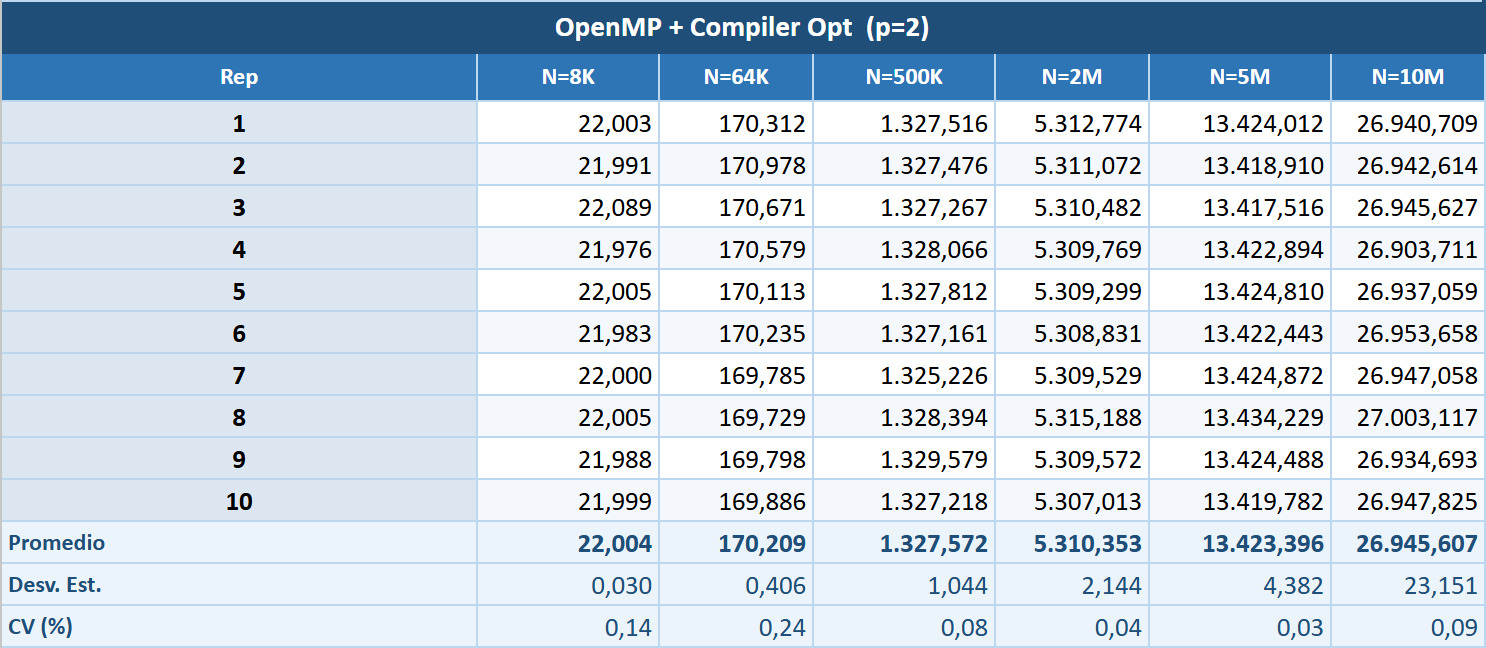
\includegraphics[width=1\textwidth]{images/results/tables/time_omp_opt_2.png}
   \caption{Tiempos de ejecución del algoritmo paralelo con OpenMP utilizando 2 hilos y optimización por compilador}
\end{table}

\begin{table}[H]
   \centering
   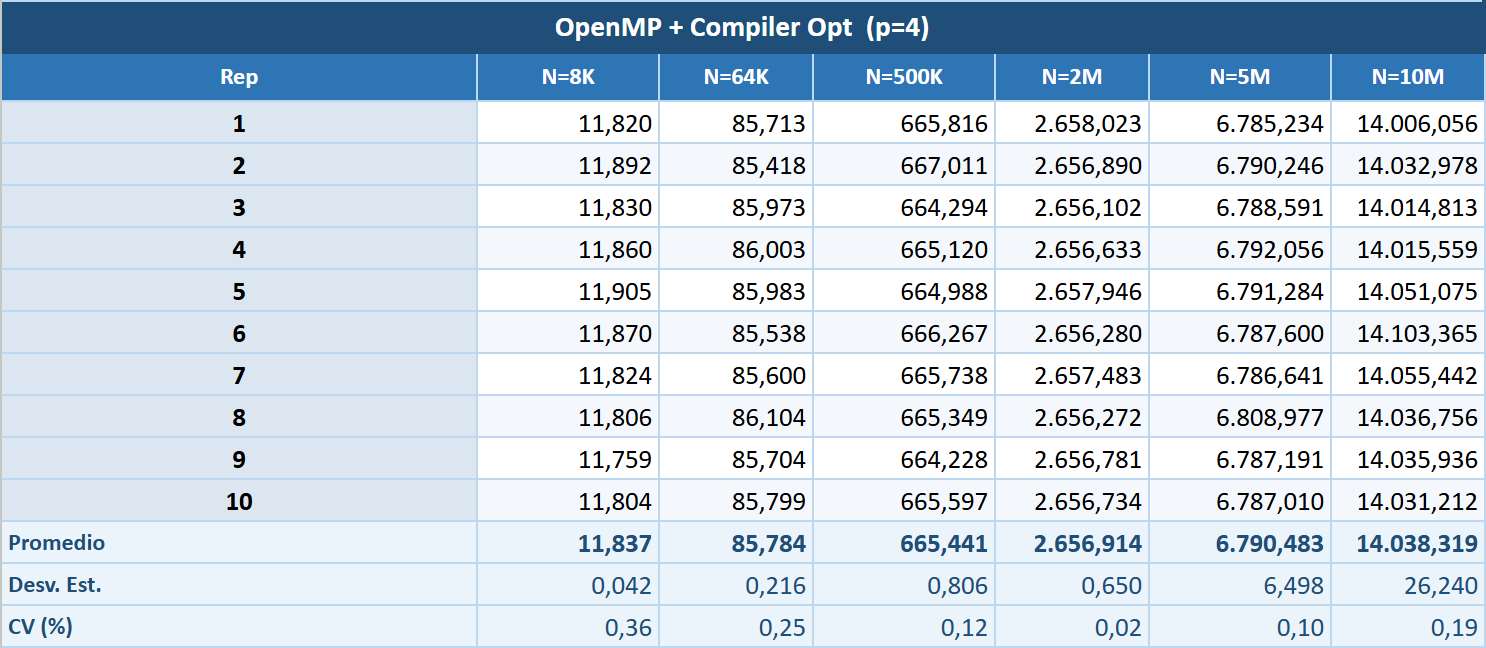
\includegraphics[width=1\textwidth]{images/results/tables/time_omp_opt_4.png}
   \caption{Tiempos de ejecución del algoritmo paralelo con OpenMP utilizando 4 hilos y optimización por compilador}
\end{table}

\begin{table}[H]
   \centering
   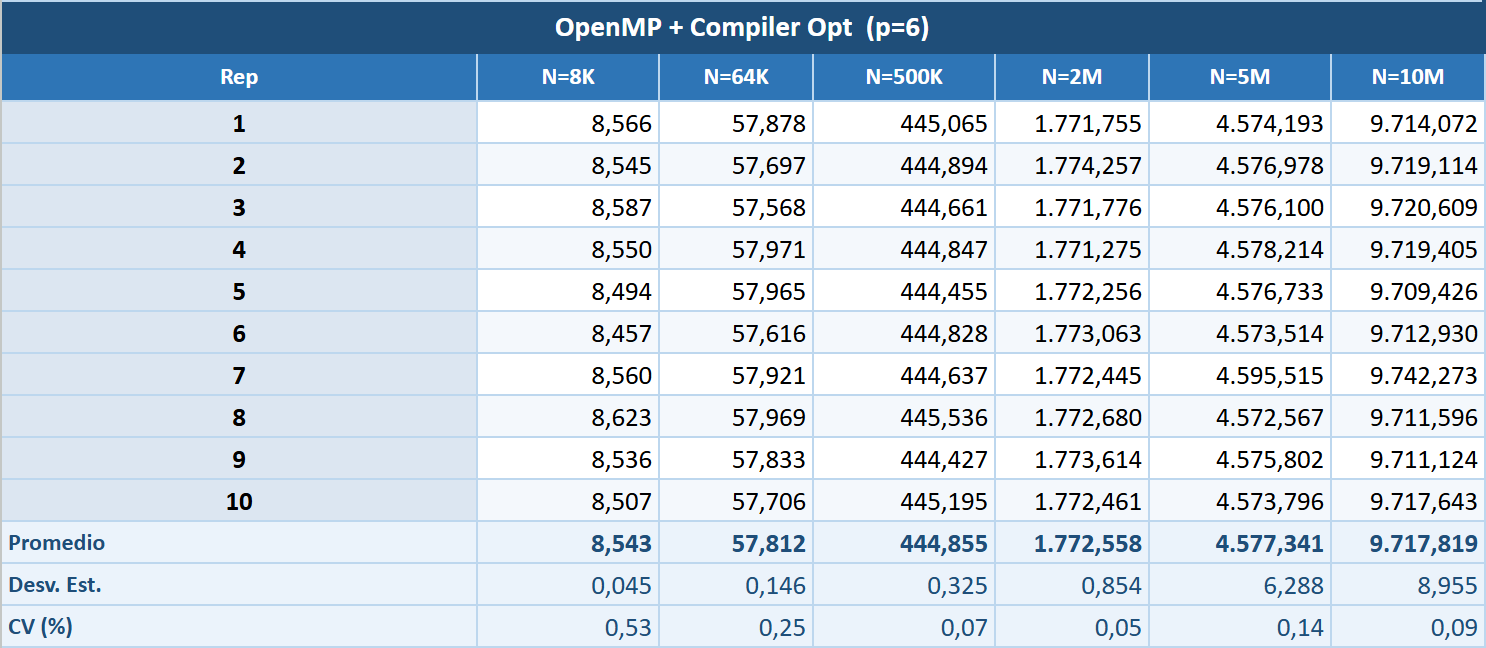
\includegraphics[width=1\textwidth]{images/results/tables/time_omp_opt_6.png}
   \caption{Tiempos de ejecución del algoritmo paralelo con OpenMP utilizando 6 hilos y optimización por compilador}
\end{table}

\begin{table}[H]
   \centering
   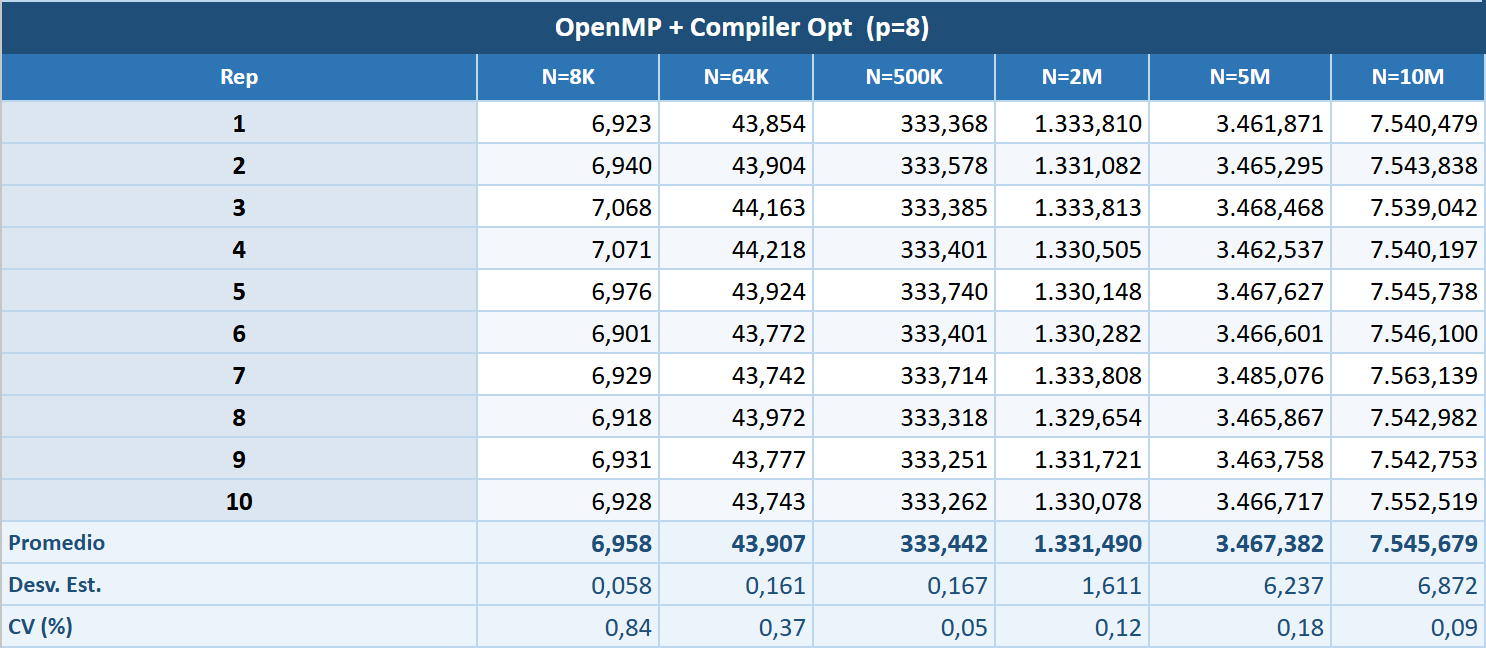
\includegraphics[width=1\textwidth]{images/results/tables/time_omp_opt_8.png}
   \caption{Tiempos de ejecución del algoritmo paralelo con OpenMP utilizando 8 hilos y optimización por compilador}
\end{table}

\begin{table}[H]
   \centering
   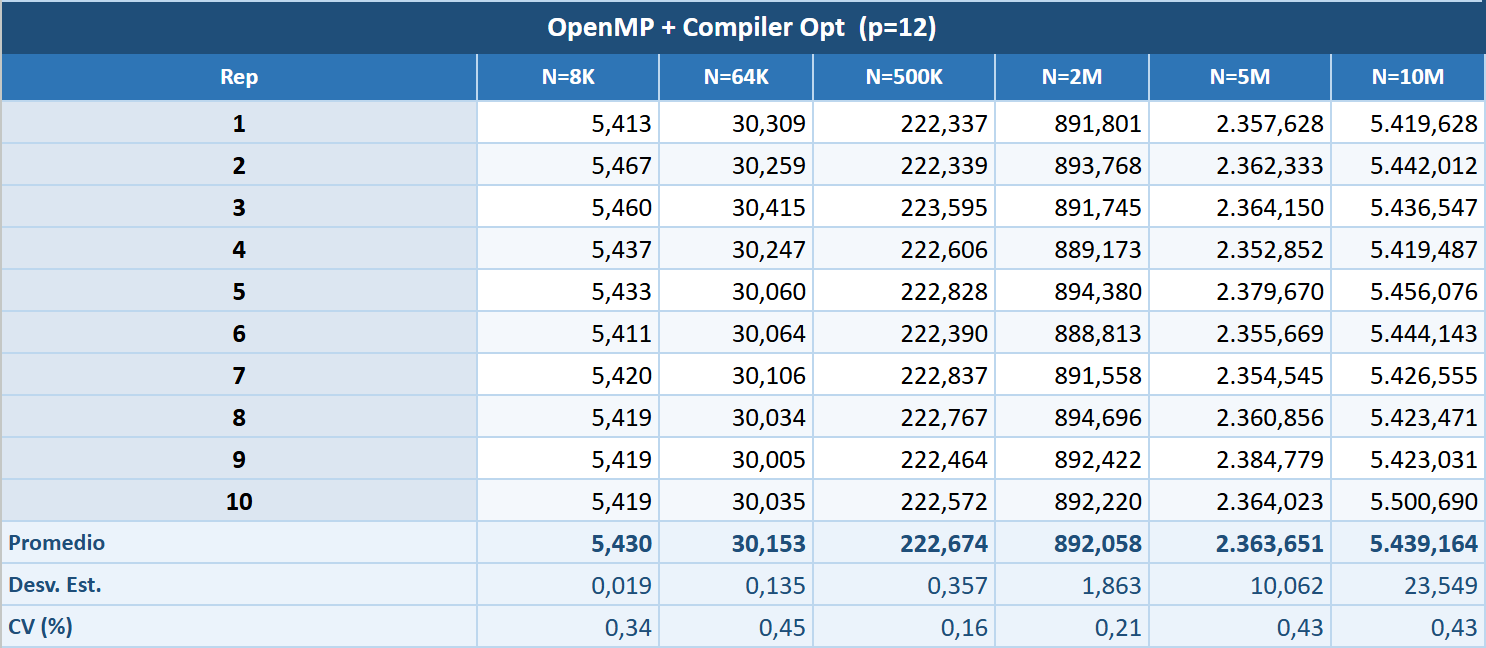
\includegraphics[width=1\textwidth]{images/results/tables/time_omp_opt_12.png}
   \caption{Tiempos de ejecución del algoritmo paralelo con OpenMP utilizando 12 hilos y optimización por compilador}
\end{table}

\begin{table}[H]
   \centering
   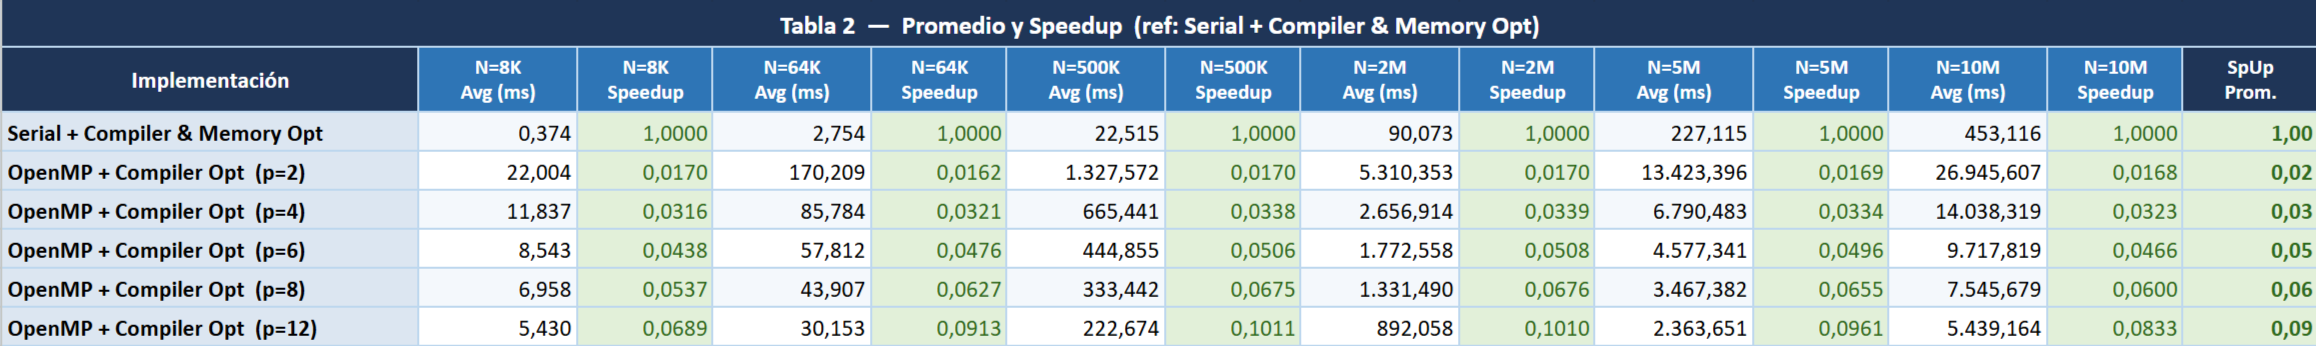
\includegraphics[width=1\textwidth]{images/results/tables/speedup_omp_opt.png}
   \caption{Speedup del algoritmo paralelo con OpenMP y optimización por compilador}
\end{table}

\begin{figure}[H]
   \centering
   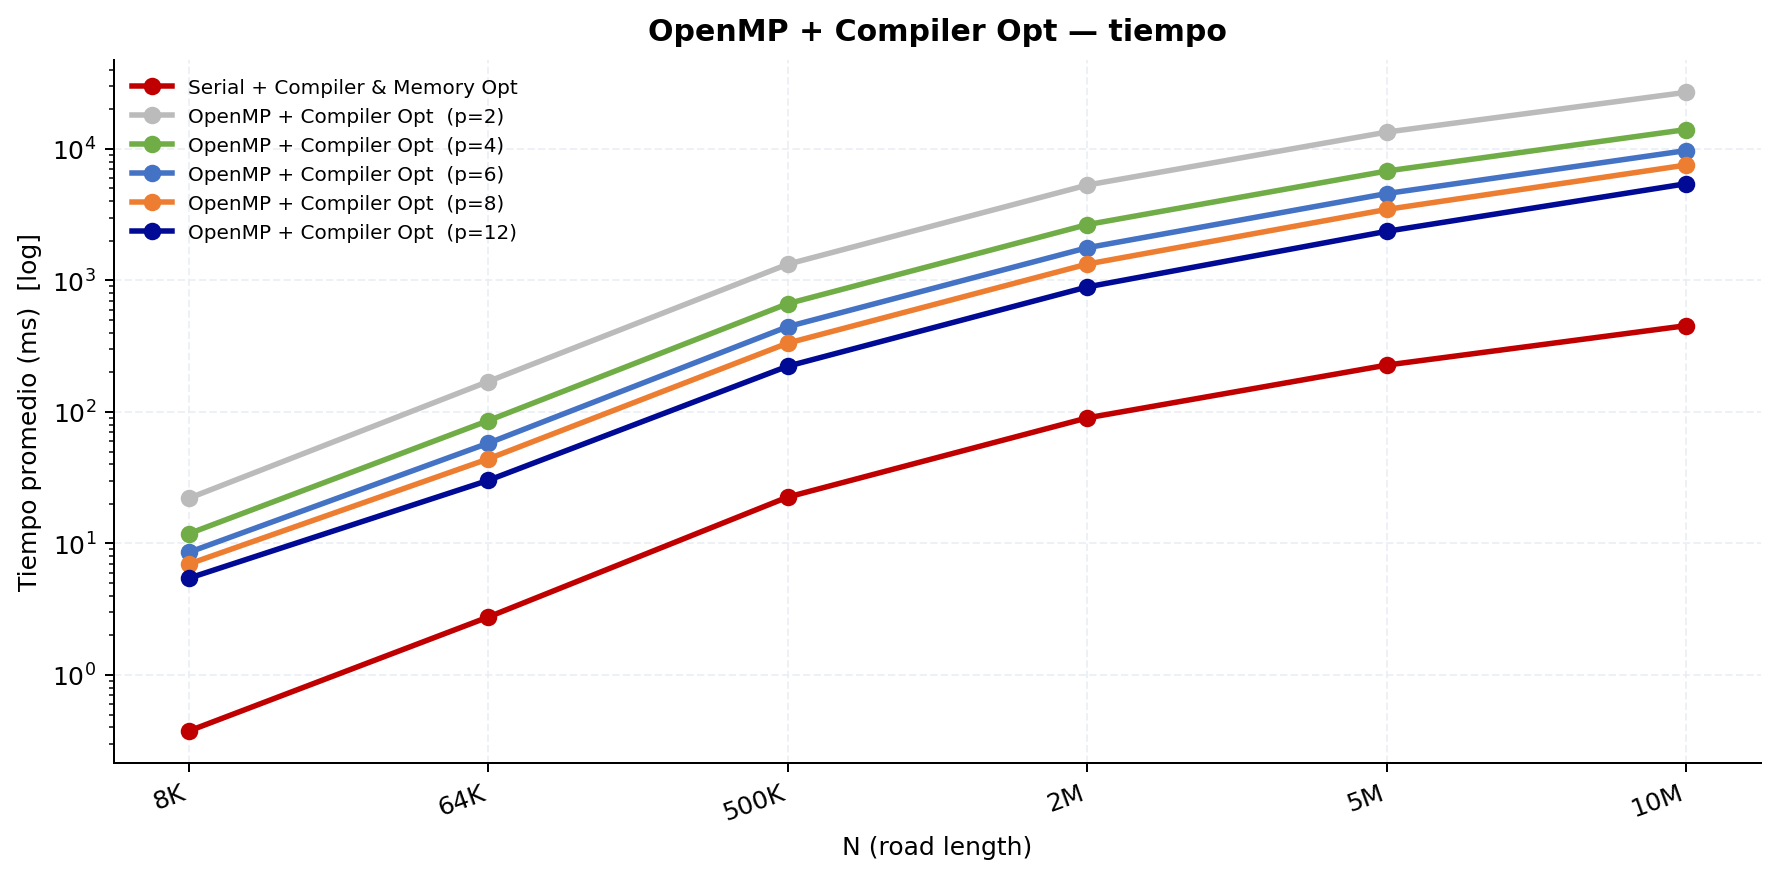
\includegraphics[width=1\textwidth]{images/results/charts/fig_omp_comp_time.png}
   \caption{Tiempos de ejecución del algoritmo paralelo con OpenMP y optimización por compilador}
\end{figure}

\begin{figure}[H]
   \centering
   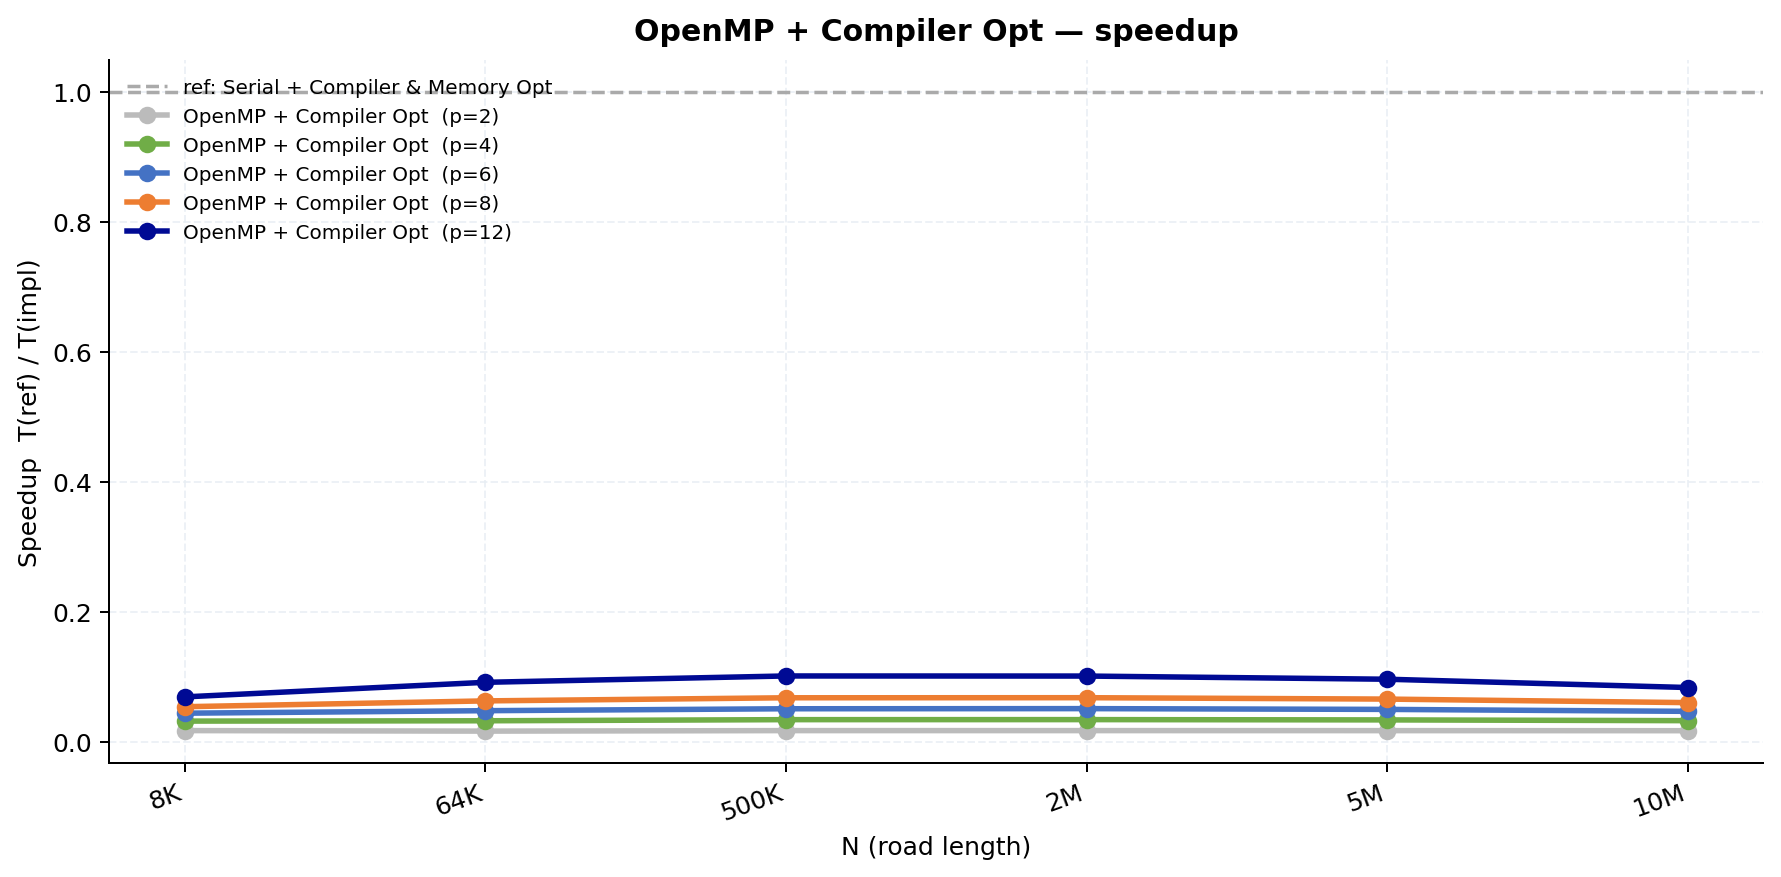
\includegraphics[width=1\textwidth]{images/results/charts/fig_omp_comp_speedup.png}
   \caption{Speedup del algoritmo paralelo con OpenMP y optimización por compilador}
\end{figure}